\documentclass[compress]{beamer}
\usepackage{ifthen,verbatim}

\newcommand{\isnote}{}
\xdefinecolor{lightyellow}{rgb}{1.,1.,0.25}
\xdefinecolor{darkblue}{rgb}{0.1,0.1,0.7}

%% Uncomment this to get annotations
%% \def\notes{\addtocounter{page}{-1}
%%            \renewcommand{\isnote}{*}
%% 	   \beamertemplateshadingbackground{lightyellow}{white}
%%            \begin{frame}
%%            \frametitle{Notes for the previous page (page \insertpagenumber)}
%%            \itemize}
%% \def\endnotes{\enditemize
%% 	      \end{frame}
%%               \beamertemplateshadingbackground{white}{white}
%%               \renewcommand{\isnote}{}}

%% Uncomment this to not get annotations
\def\notes{\comment}
\def\endnotes{\endcomment}

\setbeamertemplate{navigation symbols}{}
\setbeamertemplate{headline}{\mbox{ } \hfill
\begin{minipage}{5.5 cm}
\vspace{-0.75 cm} \small
\end{minipage} \hfill
\begin{minipage}{4.5 cm}
\vspace{-0.75 cm} \small
\begin{flushright}
\ifthenelse{\equal{\insertpagenumber}{1}}{}{Jim Pivarski \hspace{0.2 cm} \insertpagenumber\isnote/\pageref{numpages}}
\end{flushright}
\end{minipage}\mbox{\hspace{0.2 cm}}\includegraphics[height=1 cm]{../cmslogo} \hspace{0.1 cm} \includegraphics[height=1 cm]{../tamulogo} \hspace{0.01 cm} \vspace{-1.05 cm}}

\begin{document}
\begin{frame}
\vfill
\begin{center}
\textcolor{darkblue}{\Large Search for NMSSM $h \to a a \to 4\mu$ at the LHC}

\vfill
\begin{columns}
\column{0.4\linewidth}
\begin{center}
\large
Sergey Senkin

\vspace{0.2 cm}
Alexei Safonov

\vspace{0.2 cm}
\textcolor{darkblue}{Jim Pivarski}
\end{center}

\column{0.4\linewidth}
\begin{center}
\large
Alexander Belyaev
\end{center}
\end{columns}

\begin{columns}
\column{0.4\linewidth}
\begin{center}
\scriptsize
{\it Texas A\&M University}
\end{center}
\column{0.4\linewidth}
\begin{center}
\scriptsize
{\it University of Southampton}
\end{center}
\end{columns}

\vfill
 5 May, 2009

\end{center}
\end{frame}

%% \begin{notes}
%% \item This is the annotated version of my talk.
%% \item If you want the version that I am presenting, download the one
%% labeled ``slides'' on Indico (or just ignore these yellow pages).
%% \item The annotated version is provided for extra detail and a written
%% record of comments that I intend to make orally.
%% \item Yellow notes refer to the content on the {\it previous} page.
%% \item All other slides are identical for the two versions.
%% \end{notes}

\small

\begin{frame}
\frametitle{NMSSM Higgs sector}

\begin{itemize}\setlength{\itemsep}{0.2 cm}
\item Next-to-minimal supersymmetry (NMSSM) solves the $\mu$
  coincidence problem by promoting the $\mu$ term into a new singlet
  superfield
\item Also has a richer Higgs sector with CP-even ($h_1$, $h_2$)
  and CP-odd ($a_1$, $a_2$) scalars
\begin{itemize}
\item more parameter space survives LEP Higgs bounds \mbox{than MSSM\hspace{-1 cm}}
\item Higgs-to-Higgs decays can be significant
\end{itemize}
\item Exotic case: if $a_1$ is light (1--10~GeV) and $\mathcal{B}(h_1
  \to a_1 a_1)$ \mbox{is significant,\hspace{-1 cm}} normal detector signatures ($b\bar{b}$, $W^*W$, $\tau^+\tau^-$) do not apply
\item Previously studied: $h_1 \to a_1 a_1 \to 4\tau$/$2\tau 2\mu$ when $2m_\tau < m_{a_1} < 2m_b$
\item With a very light $m_{a_1} < 2m_\tau$ and $m_{h_1} < 114$~GeV, primary decay mode would be

\vspace{-0.5 cm}
\begin{center}
$h_1 \to a_1 a_1 \to 4\mu$
\end{center}
where LEP bounds do not apply to $h_1$ because of this exotic \\ (but very distinct!) final state
\end{itemize}
\end{frame}

\begin{frame}
\frametitle{Collider signature}

\begin{itemize}\setlength{\itemsep}{0.5 cm}
\item Two tightly-collimated $\mu^+\mu^-$ pairs, labeled 1-2 and 3-4

\begin{center} 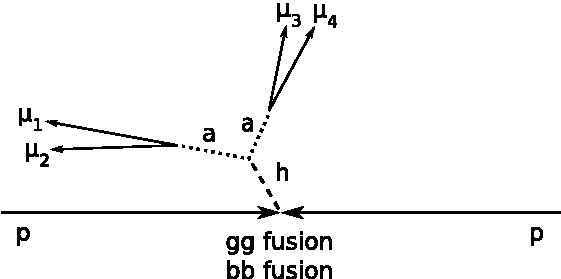
\includegraphics[width=0.75\linewidth]{signature.pdf} \end{center}

\item Leading $\mu$ $p_T > 20$~GeV: negligible background from $J/\psi$
\item Because of low backgrounds, one does not need to resort to sub-dominant vector boson fusion production for tagging
\end{itemize}
\end{frame}

\begin{frame}
\frametitle{News: D$\emptyset$ search for $h \to 4\mu$}

\begin{itemize}
\item Released upper limit on $h \to aa \to 4\mu$: {\scriptsize \tt Conference Note 5891-CONF}

{\scriptsize \tt http://www-d0.fnal.gov/Run2Physics/WWW/results/prelim/HIGGS/H67/}
\end{itemize}
\begin{columns}
\column{0.5\linewidth}
\mbox{\hspace{0.5 cm}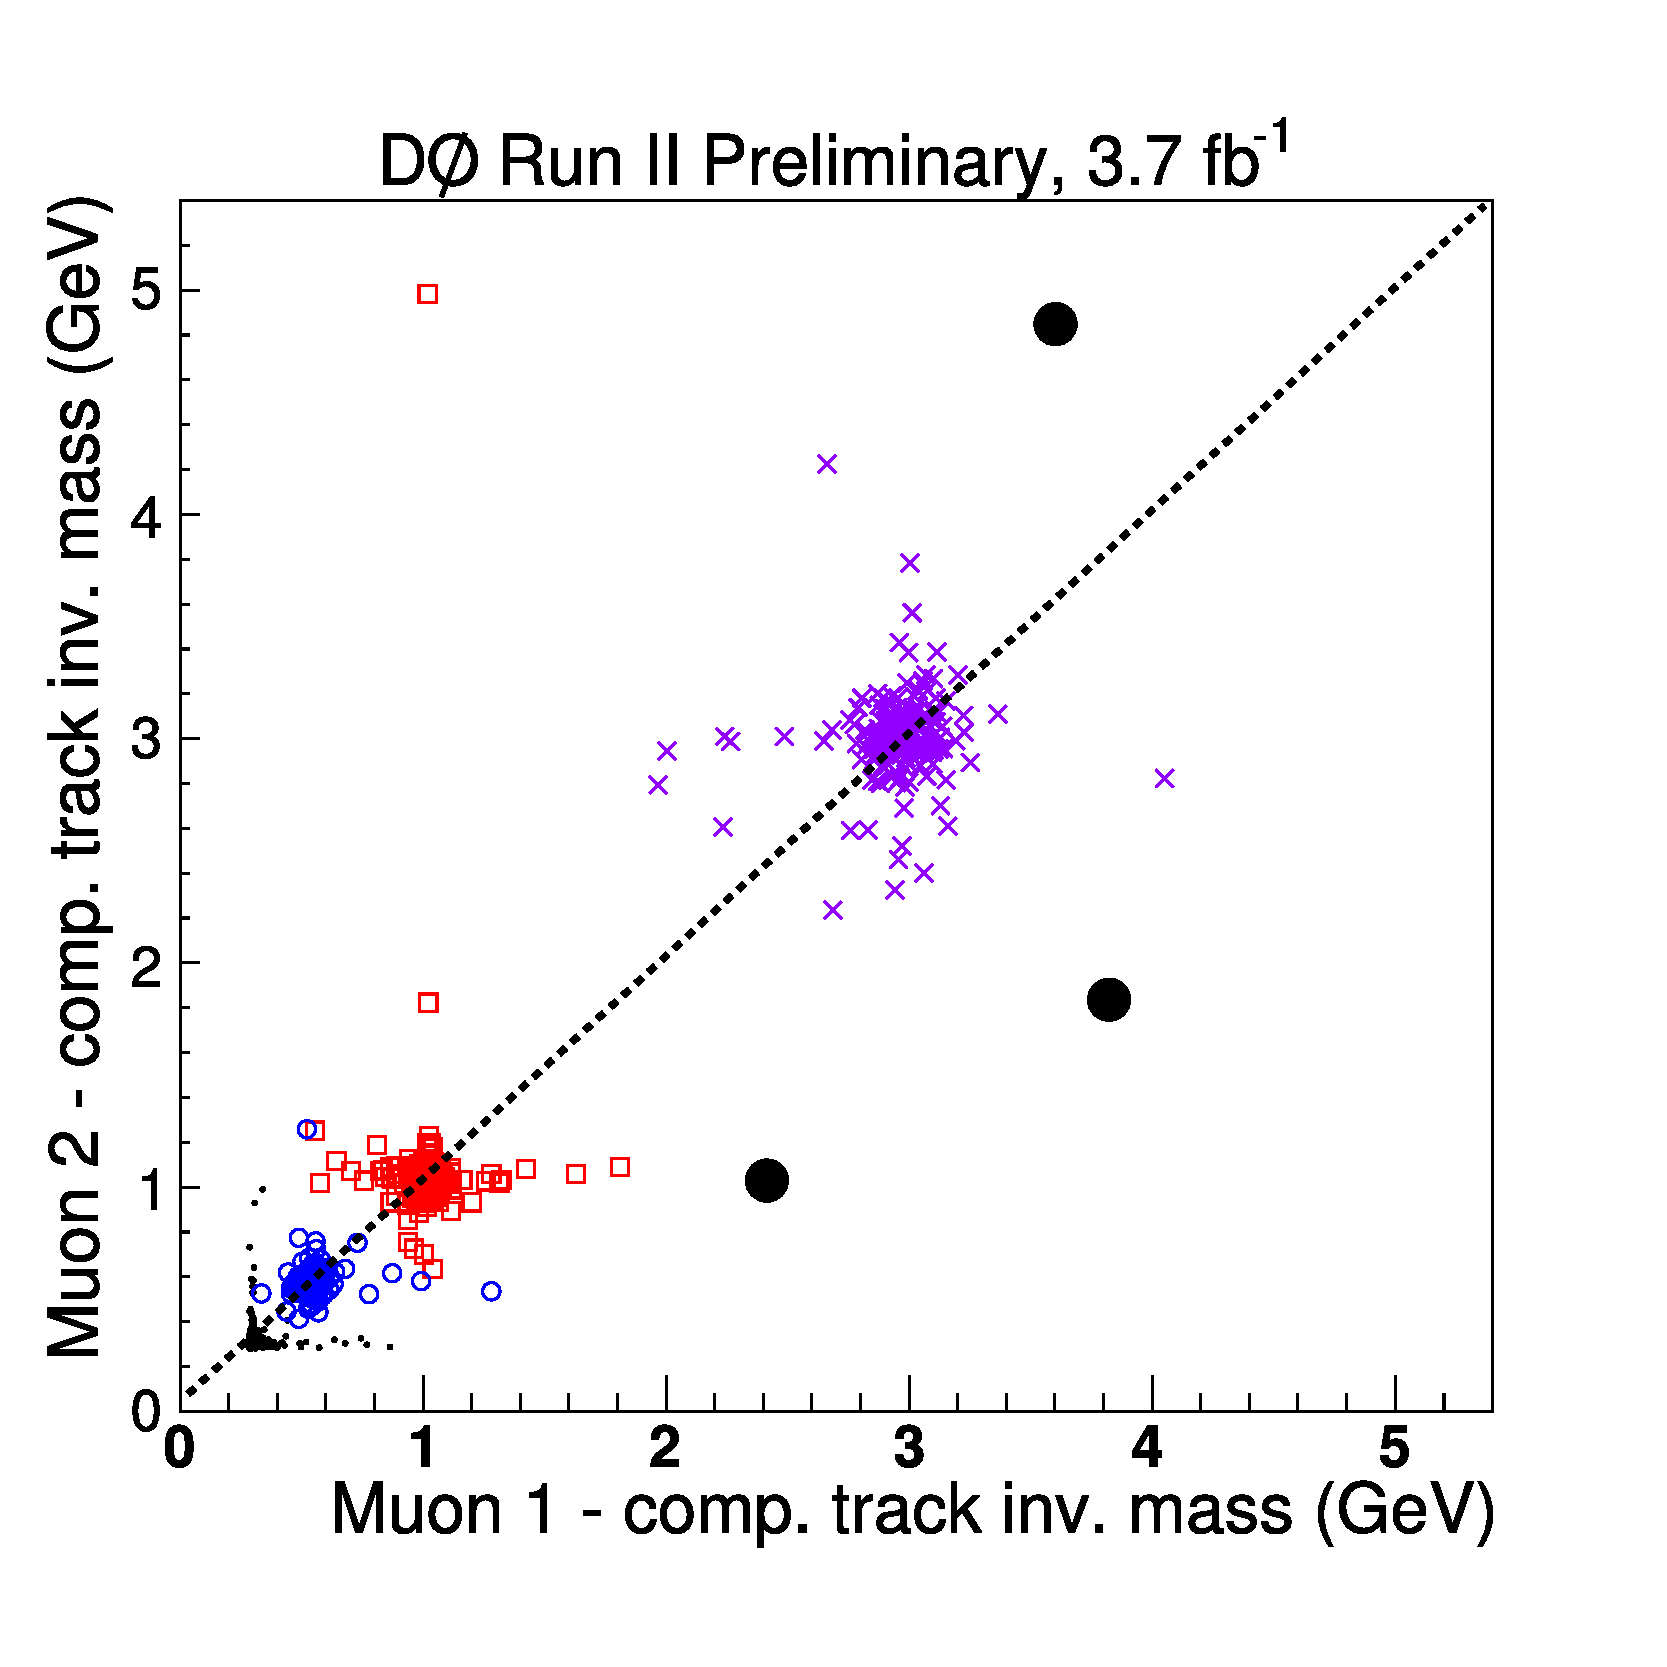
\includegraphics[width=\linewidth]{d0_search.pdf}}

\column{0.65\linewidth}
\begin{itemize}
\item Insufficient muon granularity to resolve two muons with a small opening angle
\item Paired identified muon with \\ ``companion track'' in narrow cone
\item muon $+$ track pair isolated to reduce backgrounds
\item $m_a$ = \textcolor{blue}{0.5~GeV,} \textcolor{red}{1~GeV,} and \textcolor{violet}{3~GeV} simulations and 3 surviving data events shown in $m_{12}$ vs.\ $m_{34}$ plane
\end{itemize}
\end{columns}
\begin{itemize}
\item Assuming an $h$ production cross-section of 1~pb, D$\emptyset$ sets an upper limit on $\mathcal{B}(h \to aa)$ at 10\%
\end{itemize}
\end{frame}

\begin{frame}
\frametitle{4$\mu$ model is not ruled out}

\vfill
$h_1$ has a non-standard coupling to $gg$, $b\bar{b}$; NMSSM prefers \mbox{low cross-section\hspace{-1 cm}}

\vfill
\begin{columns}
\column{0.7\linewidth}
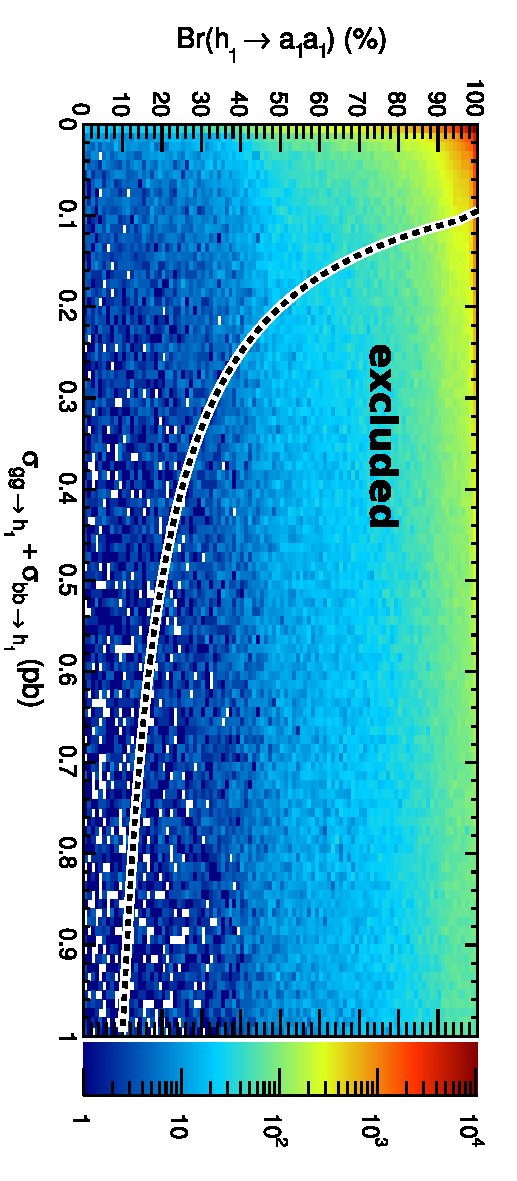
\includegraphics[height=\linewidth, angle=90]{br_vs_production2.pdf}

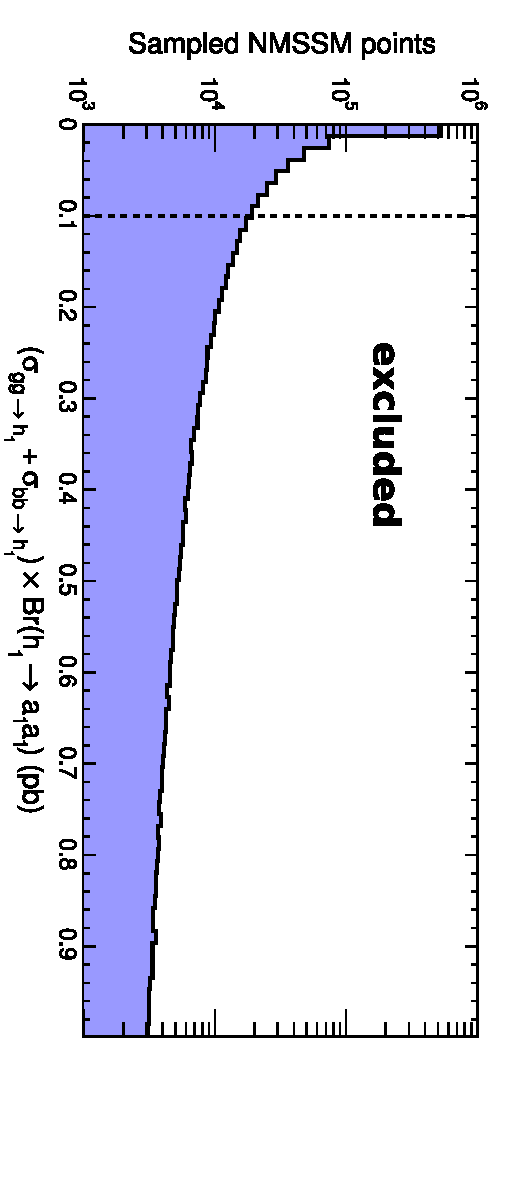
\includegraphics[height=\linewidth, angle=90]{br_vs_production4.pdf}

\column{0.3\linewidth}

\mbox{NMSSMTools uniform\hspace{-0.5 cm}} scan over parameters:
\begin{center}
$0 < \kappa/\lambda < 0.8$

\vspace{0.1 cm}
$0 < \lambda < 0.1$

\vspace{0.1 cm}
$-0.1 < A_\kappa < 0$~GeV

\vspace{0.1 cm}
$0 < A_\lambda < 4$~TeV

\vspace{0.1 cm}
$100 < \mu < 200$~GeV

\vspace{0.1 cm}
$10 < \tan\beta < 60$
\end{center}

\vspace{0.3 cm}
Cross-section $\ll$ limit for most parameters

\vspace{0.3 cm}
(note log scales)
\end{columns}
\end{frame}

\begin{frame}
\frametitle{Branching fractions study}

\vspace{0.25 cm}
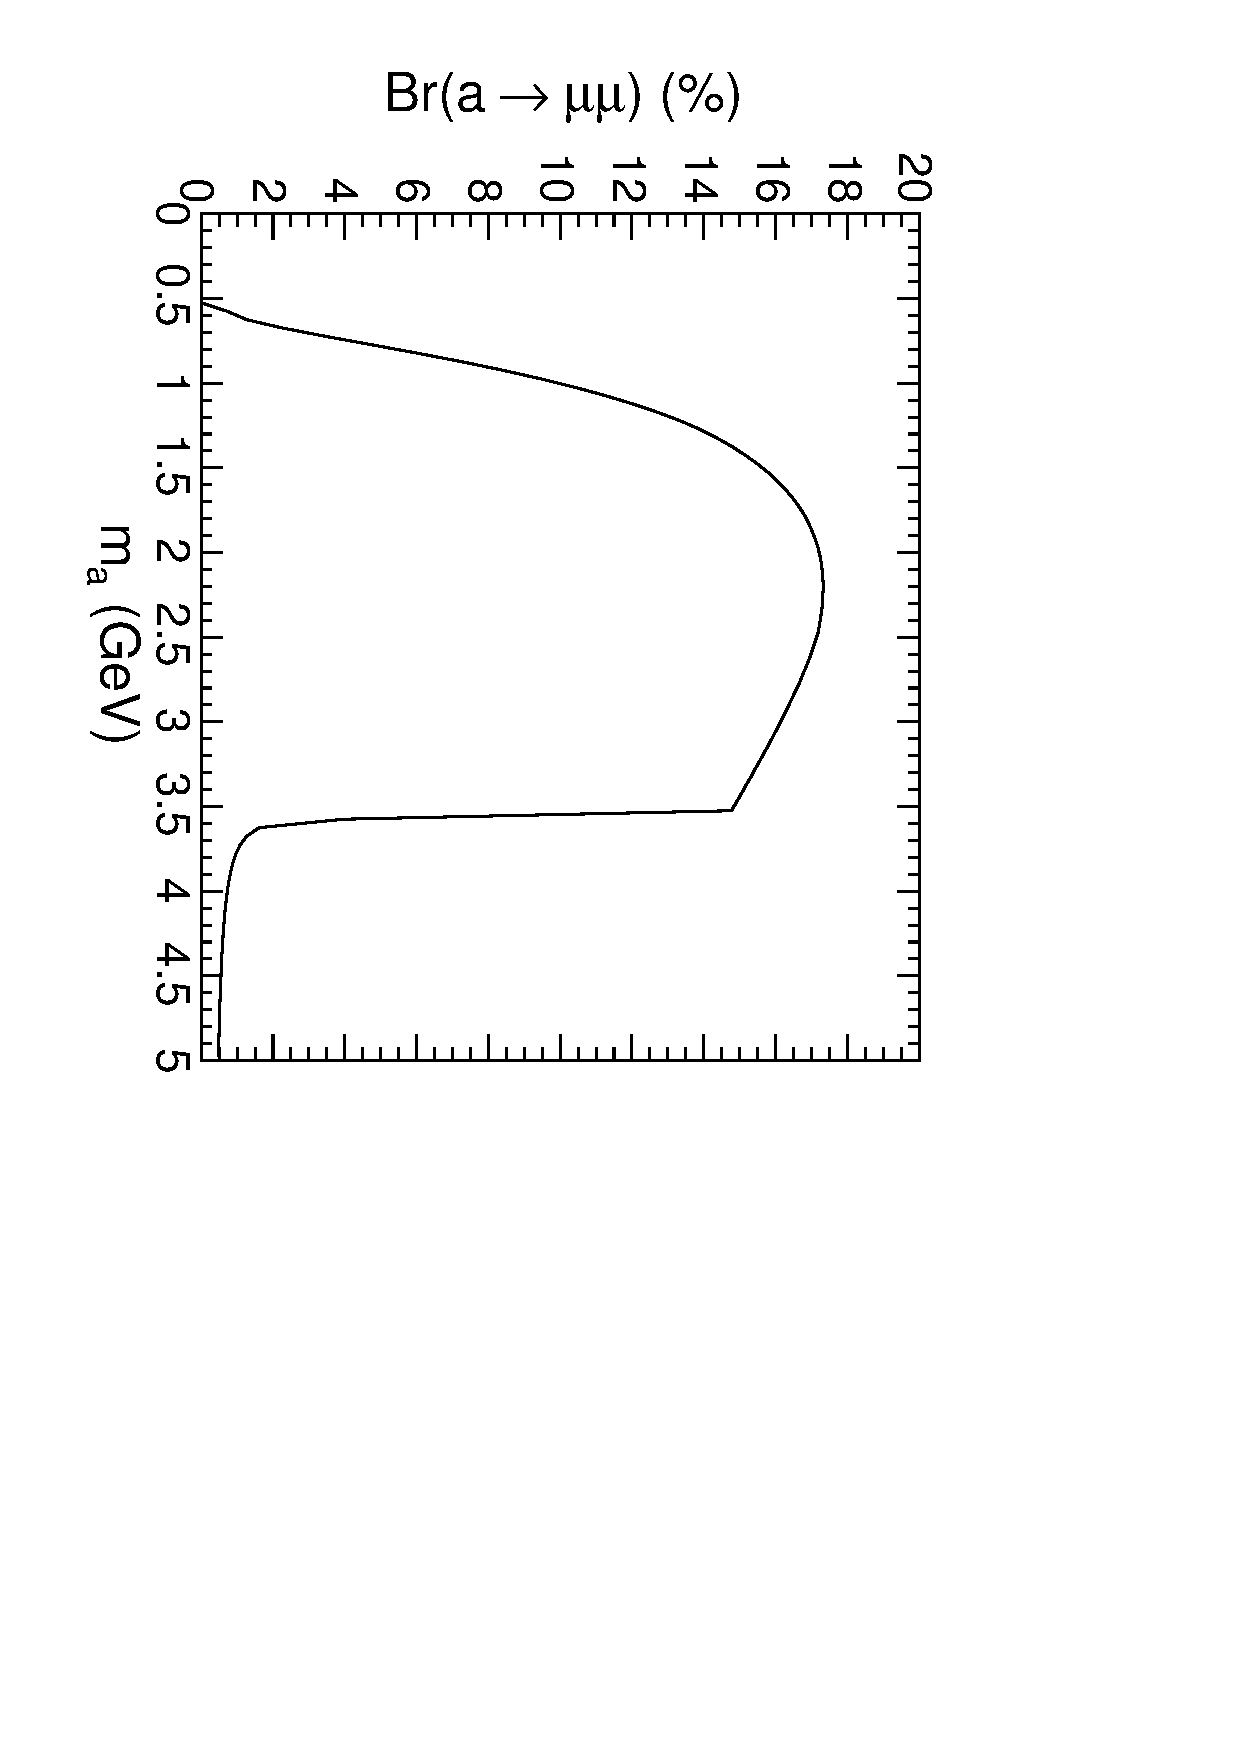
\includegraphics[height=0.33\linewidth, angle=90]{branching_fractions_plot_widescan.pdf} \hfill
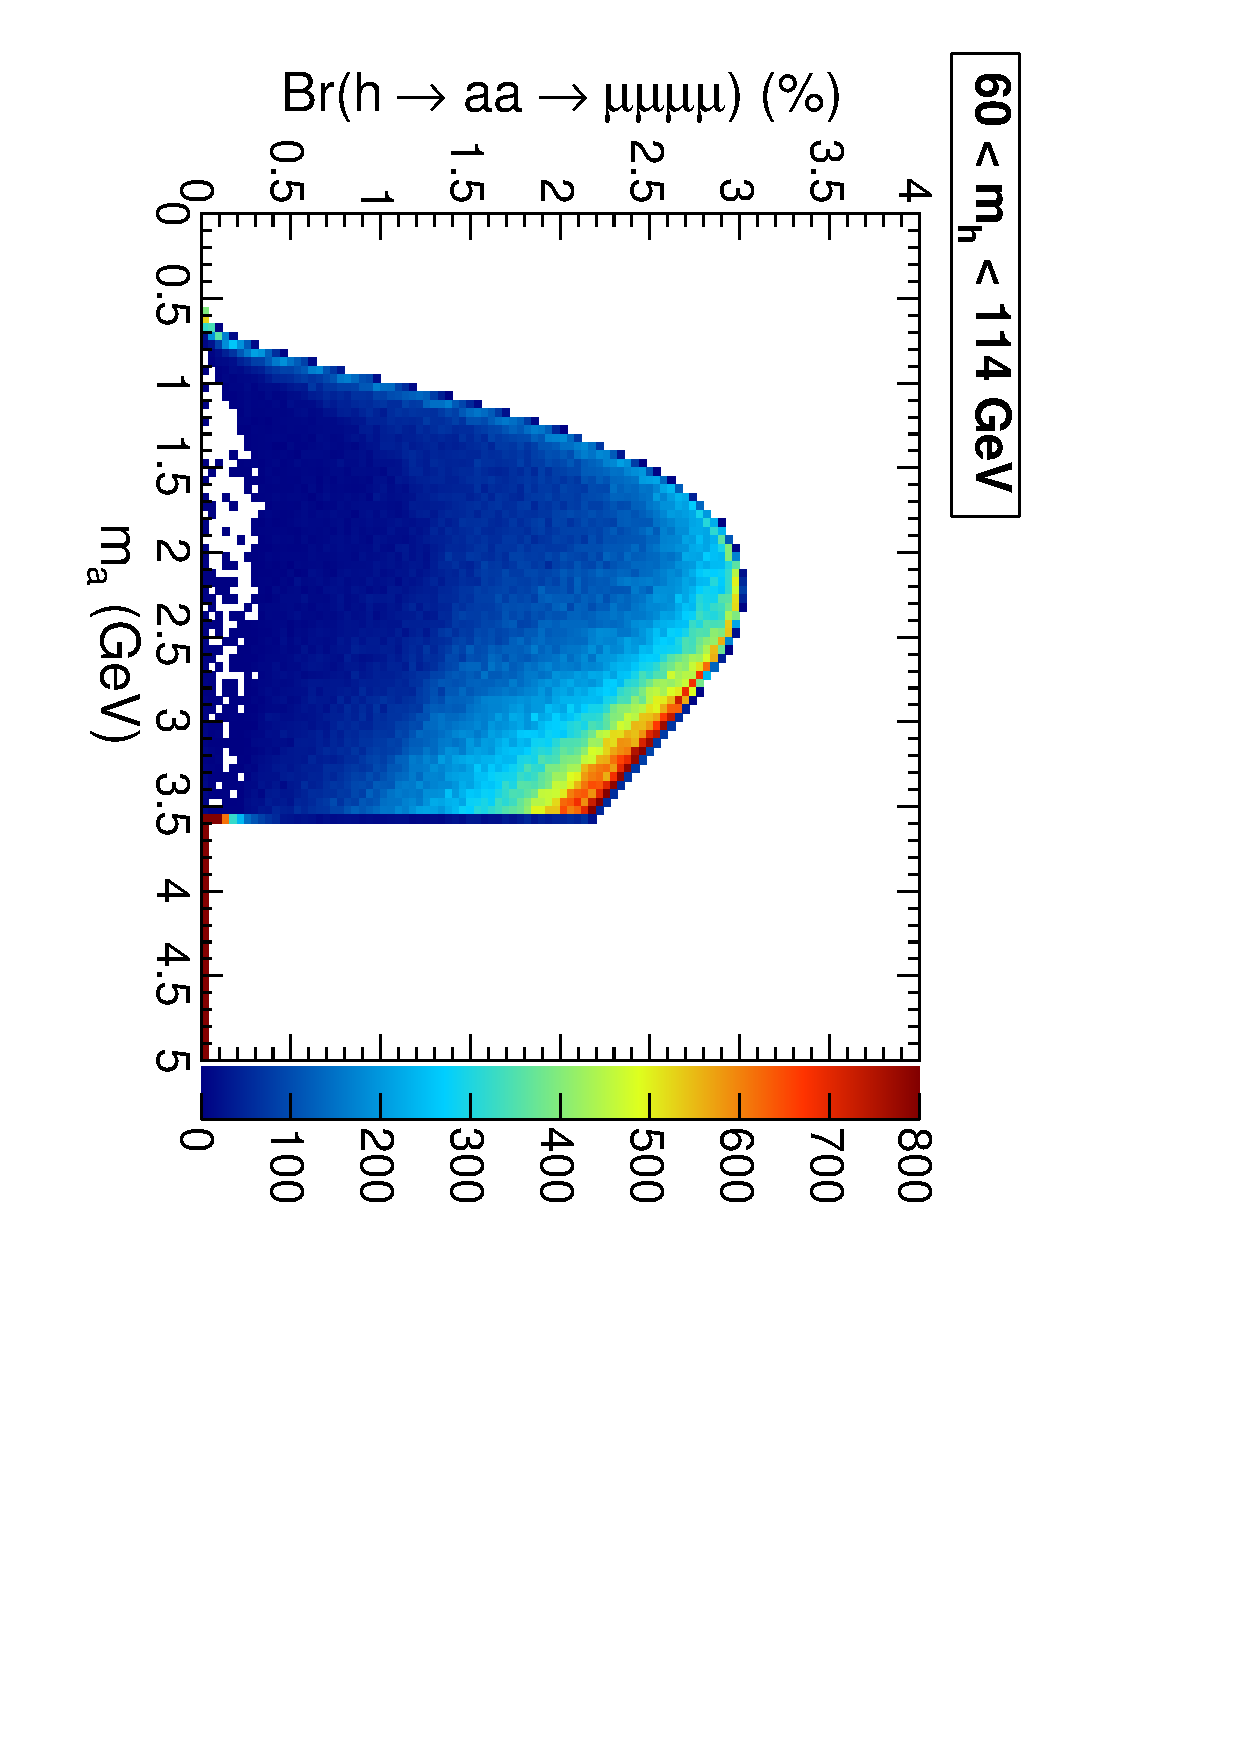
\includegraphics[height=0.33\linewidth, angle=90]{brh4mu_pmass1_widescan.pdf} \hfill
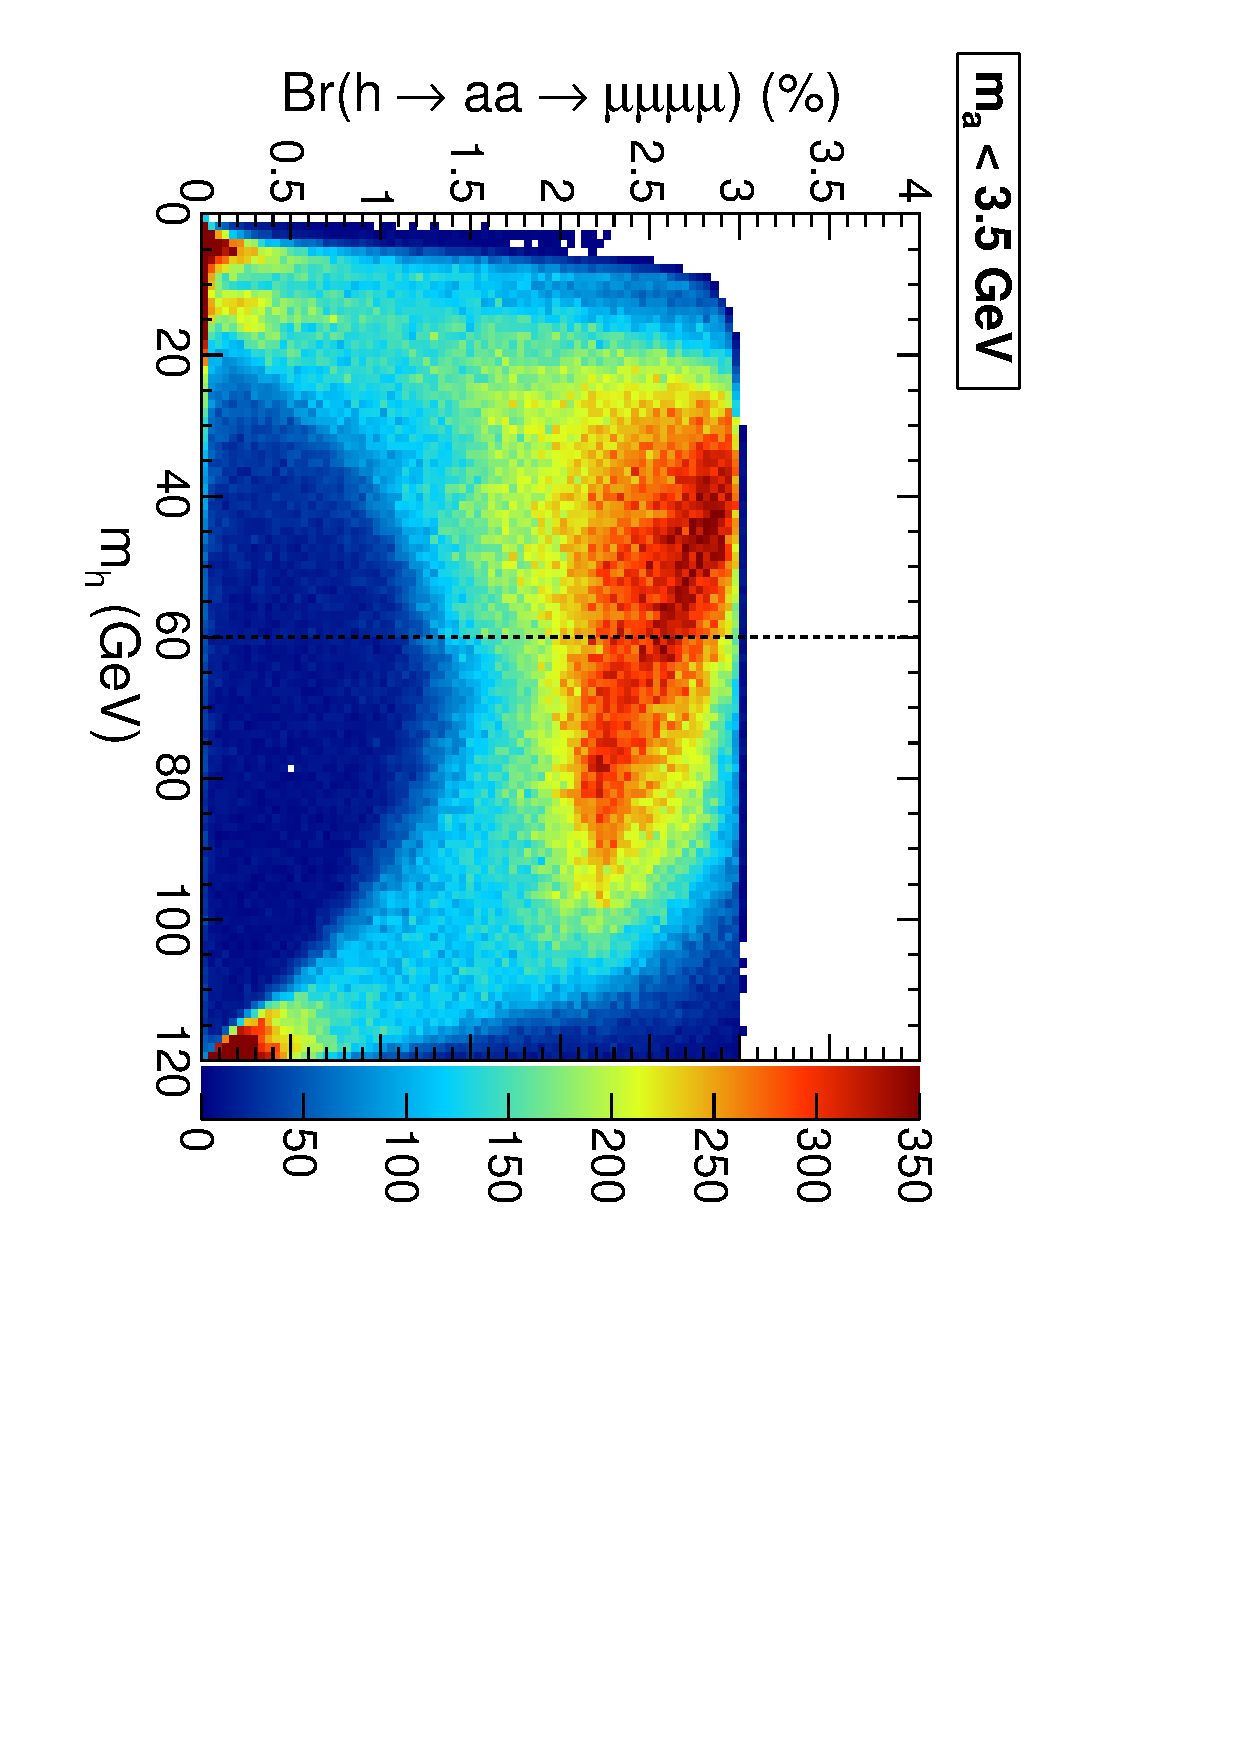
\includegraphics[height=0.33\linewidth, angle=90]{brh4mu_smass1_widescan.pdf}

\vspace{-0.4 cm}
\begin{itemize}
\item Significant for $1\mbox{ GeV} < m_a < 2m_\tau = 3.55$~GeV and $m_h < 114$~GeV
\end{itemize}

\begin{columns}
\column{0.55\linewidth}
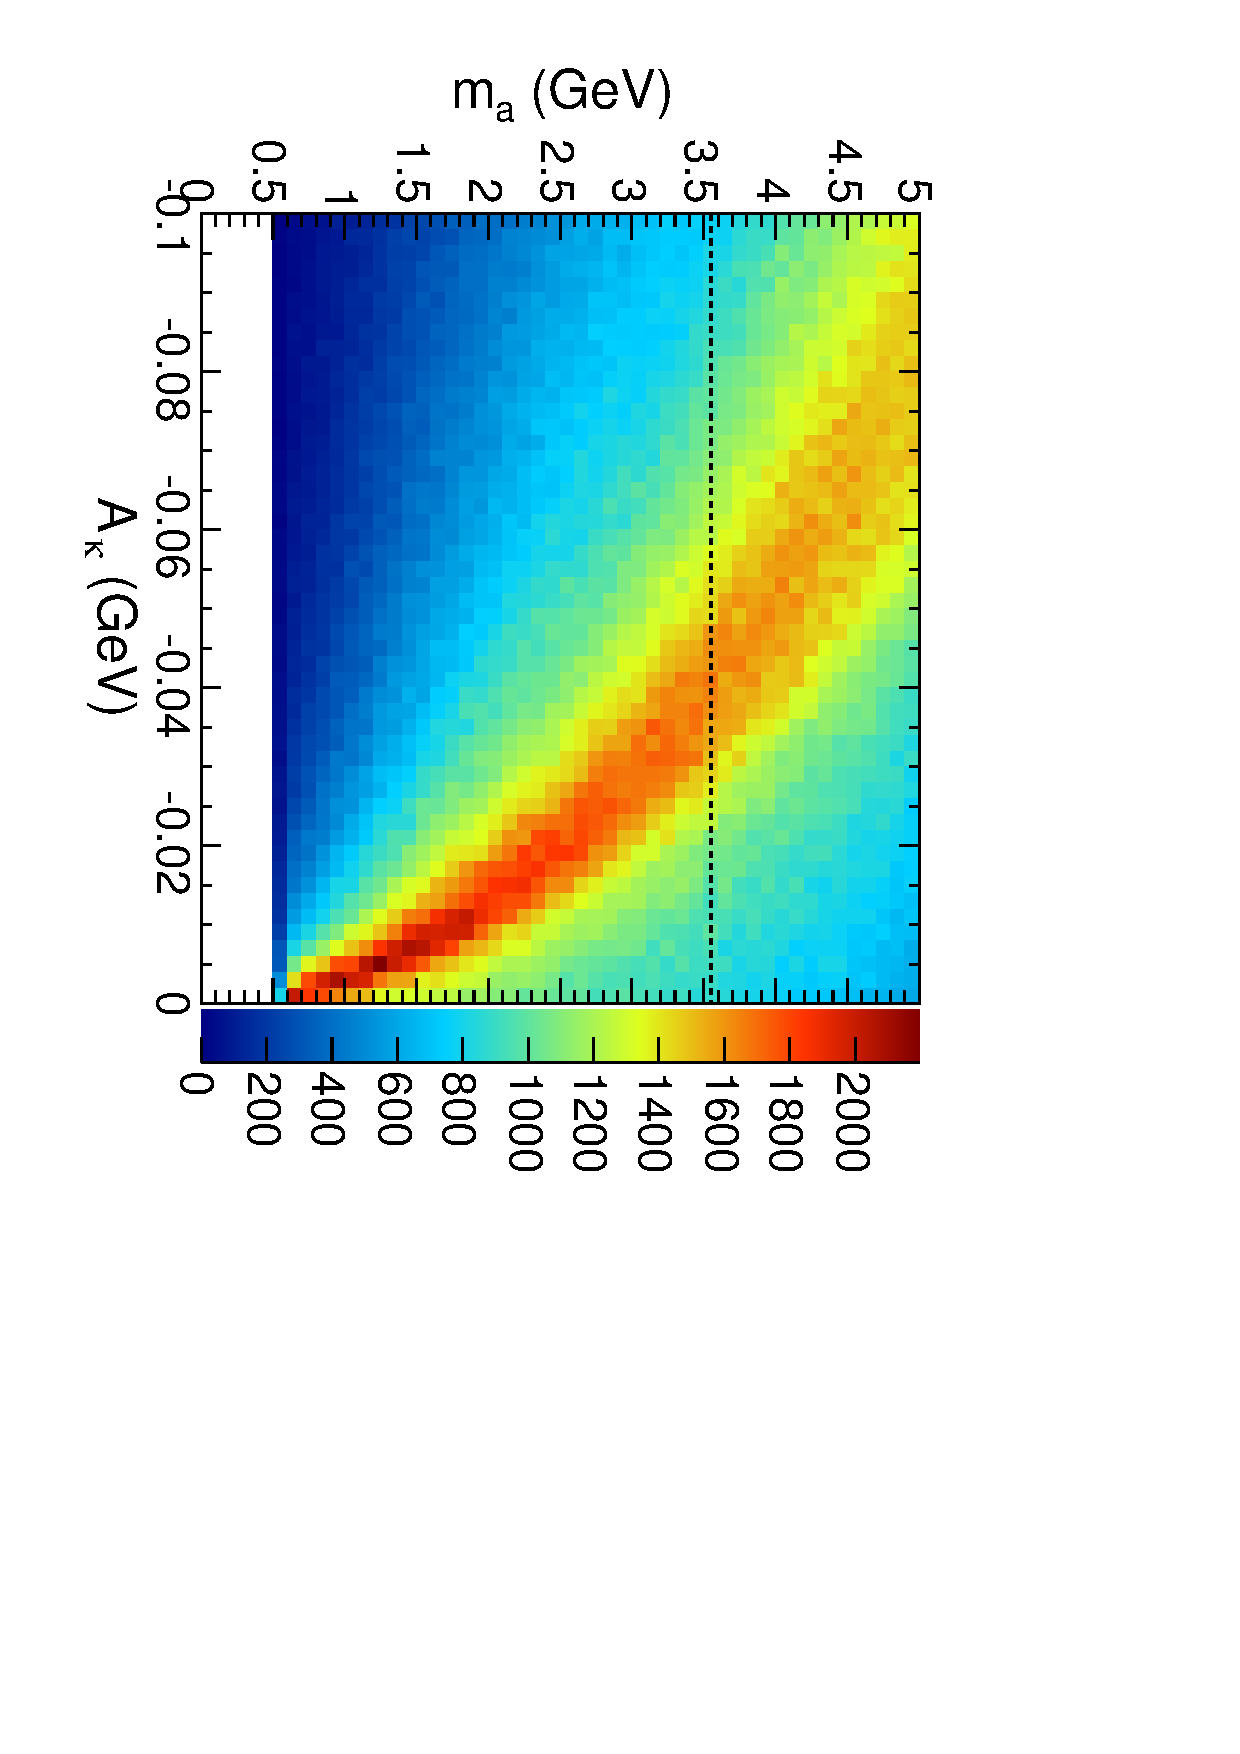
\includegraphics[height=0.5\linewidth, angle=90]{pmass1_Akappa_widescan.pdf}
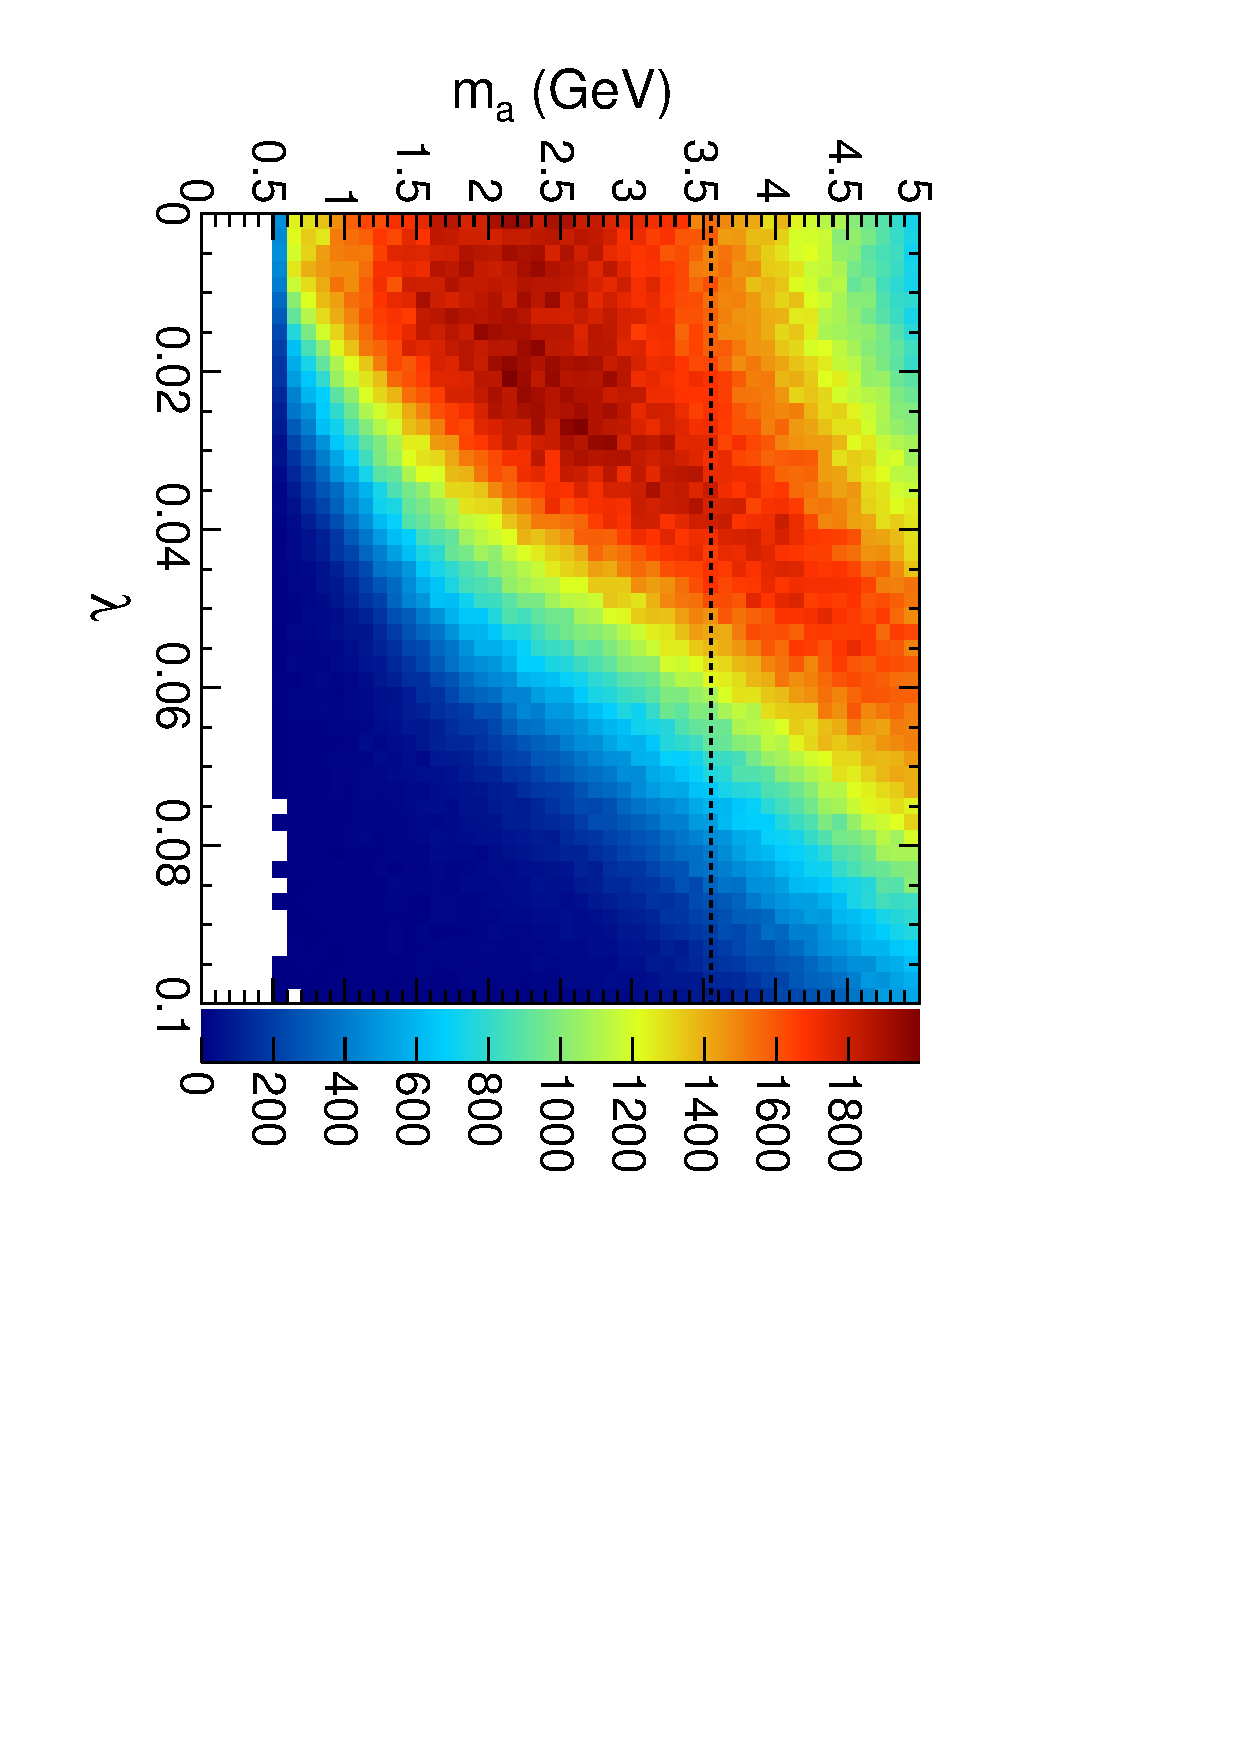
\includegraphics[height=0.5\linewidth, angle=90]{pmass1_lambda_widescan.pdf}

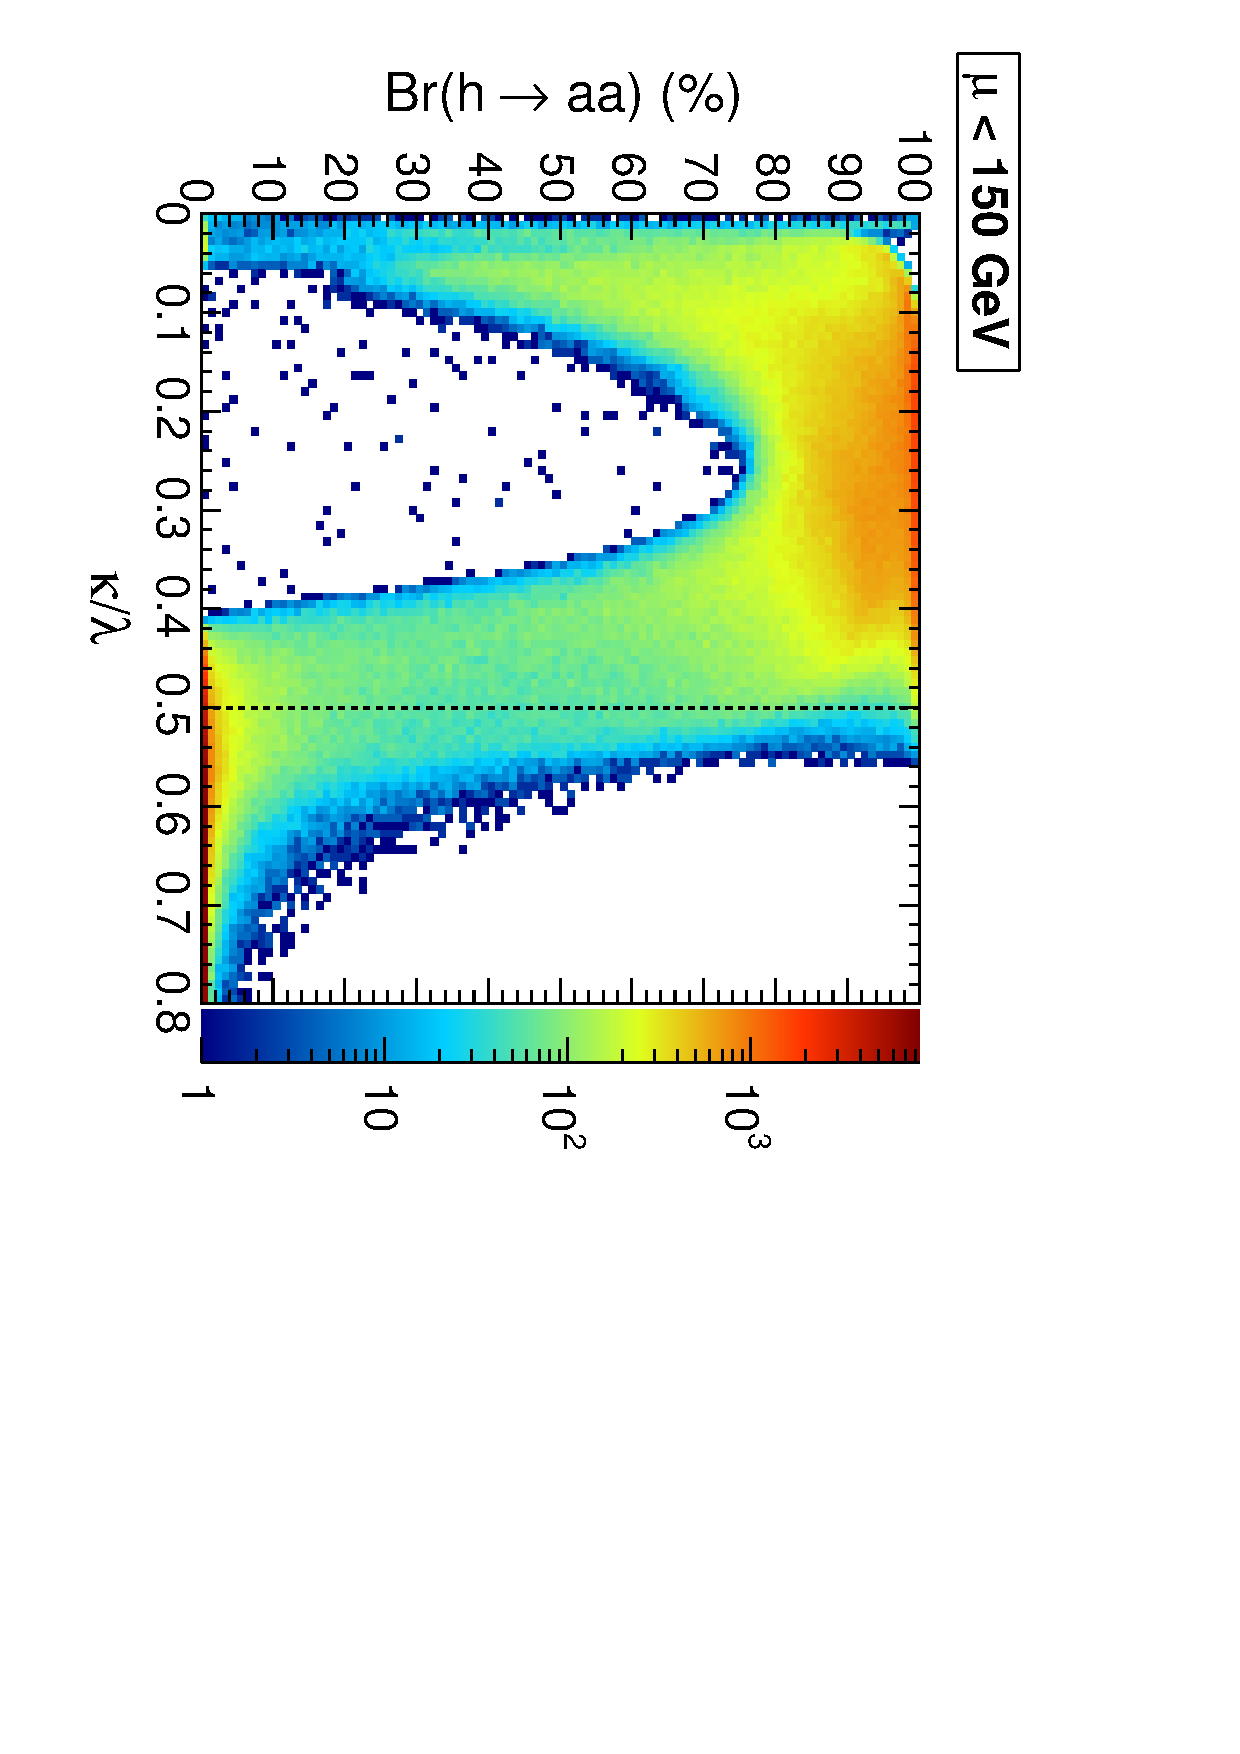
\includegraphics[height=0.5\linewidth, angle=90]{koverl_widescan.pdf}
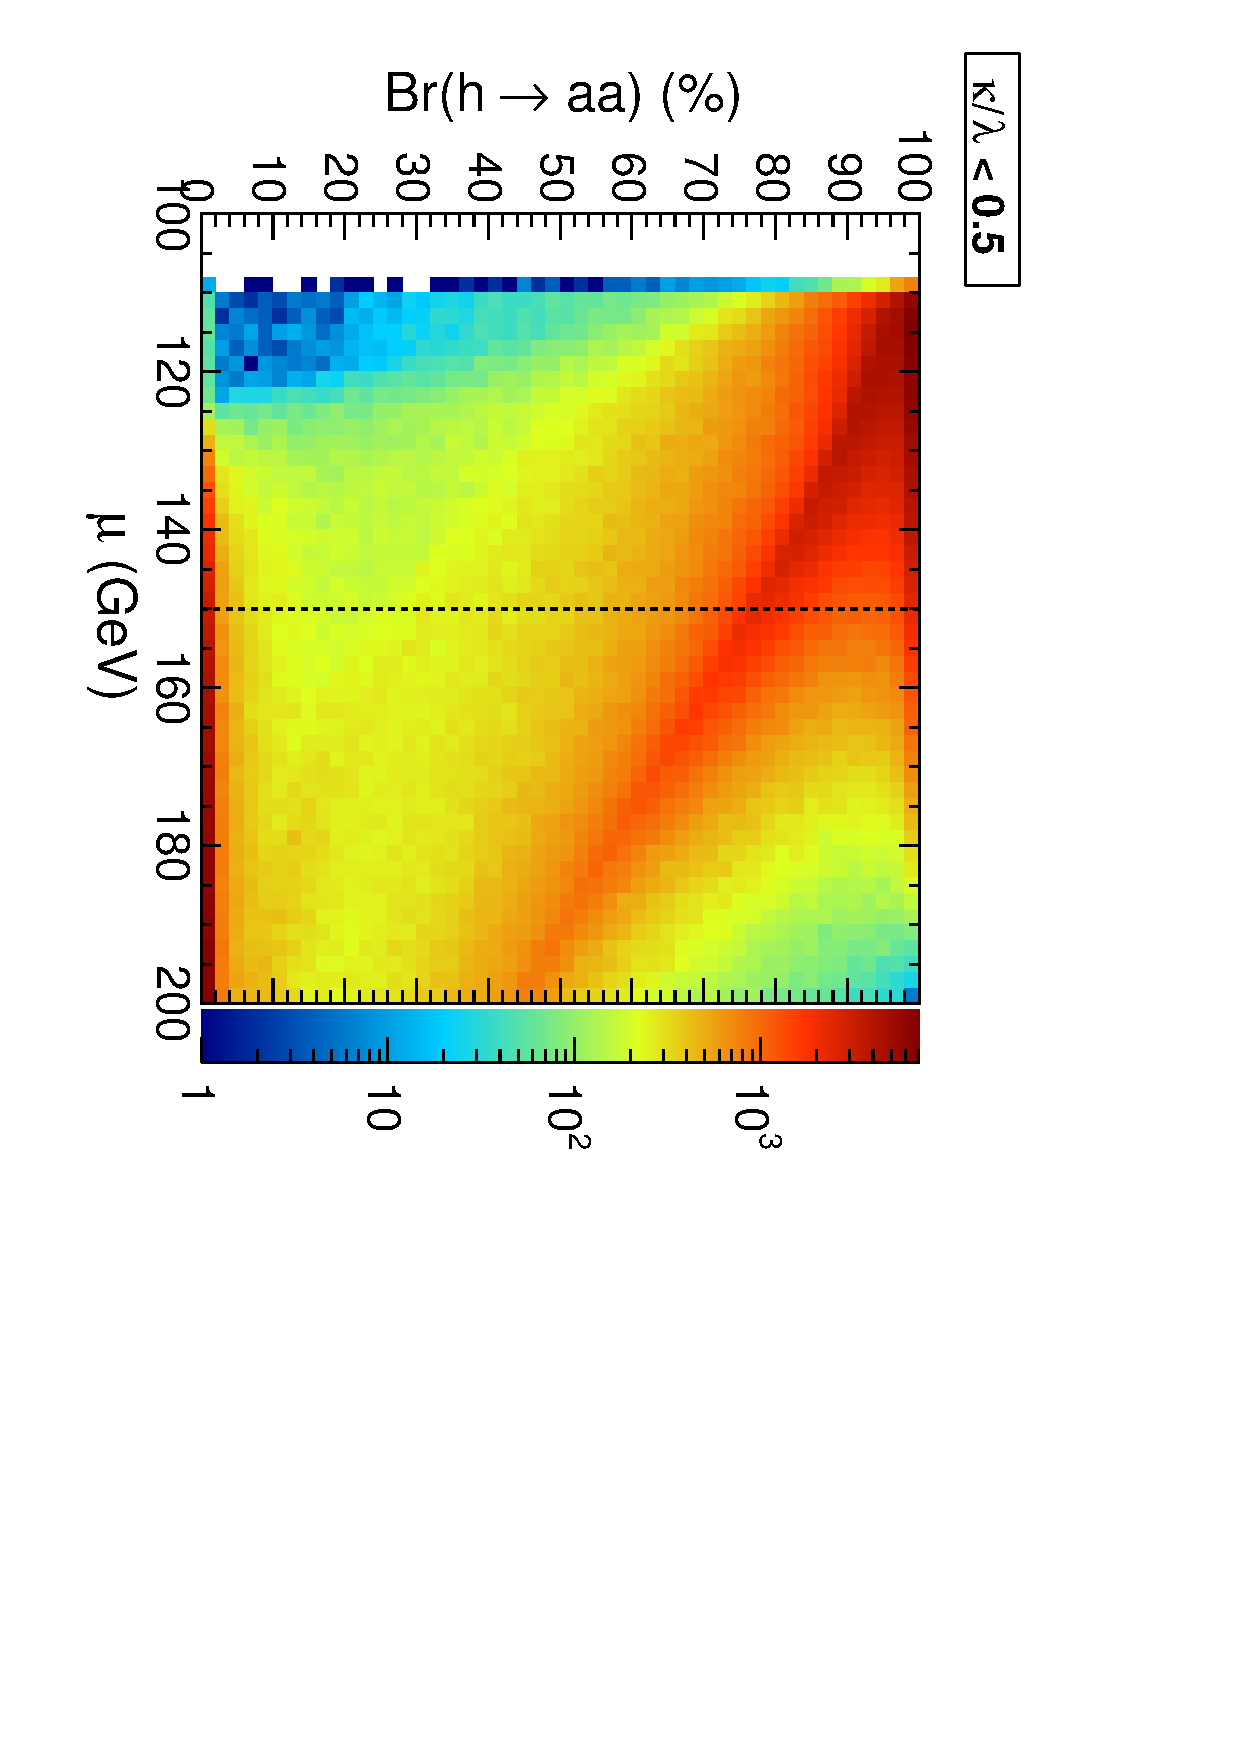
\includegraphics[height=0.5\linewidth, angle=90]{mu_widescan.pdf}

\column{0.5\linewidth}
\begin{itemize}
\item $A_\kappa$ and $\lambda$ must be small for $m_a < 2m_\tau$ {\scriptsize (linear scale)}

\vspace{0.85 cm}

\item $\kappa/\lambda$ and $\mu$ must be small for $\mathcal{B}(h \to aa) \gtrsim 50$\% {\scriptsize (log scale)}

\item Different regions have qualitatively different behvaior
\end{itemize}
\end{columns}
\end{frame}

\begin{frame}
\frametitle{Sensitivity at LHC}

\begin{itemize}
\item CMS as a benchmark
\item Finer granularity in muon identification than D$\emptyset$: require 4 muons
\begin{itemize}\setlength{\itemsep}{0.1 cm}
\item highest $p_T > 20$~GeV, all others $> 5$~GeV
\item $|\eta| < 2.4$
\item minimize ${\Delta R(\mu_1\mbox{, }\mu_2)}^2 + {\Delta R(\mu_3\mbox{, }\mu_4)}^2$ to pair 1-2 and 3-4
\item simultaneously fit $m_{12}$, $m_{34}$, and $m_{1234}$ spectra
\end{itemize}
\item Simulated distributions with detector resolution (CMS TDR):
\end{itemize}

\vfill
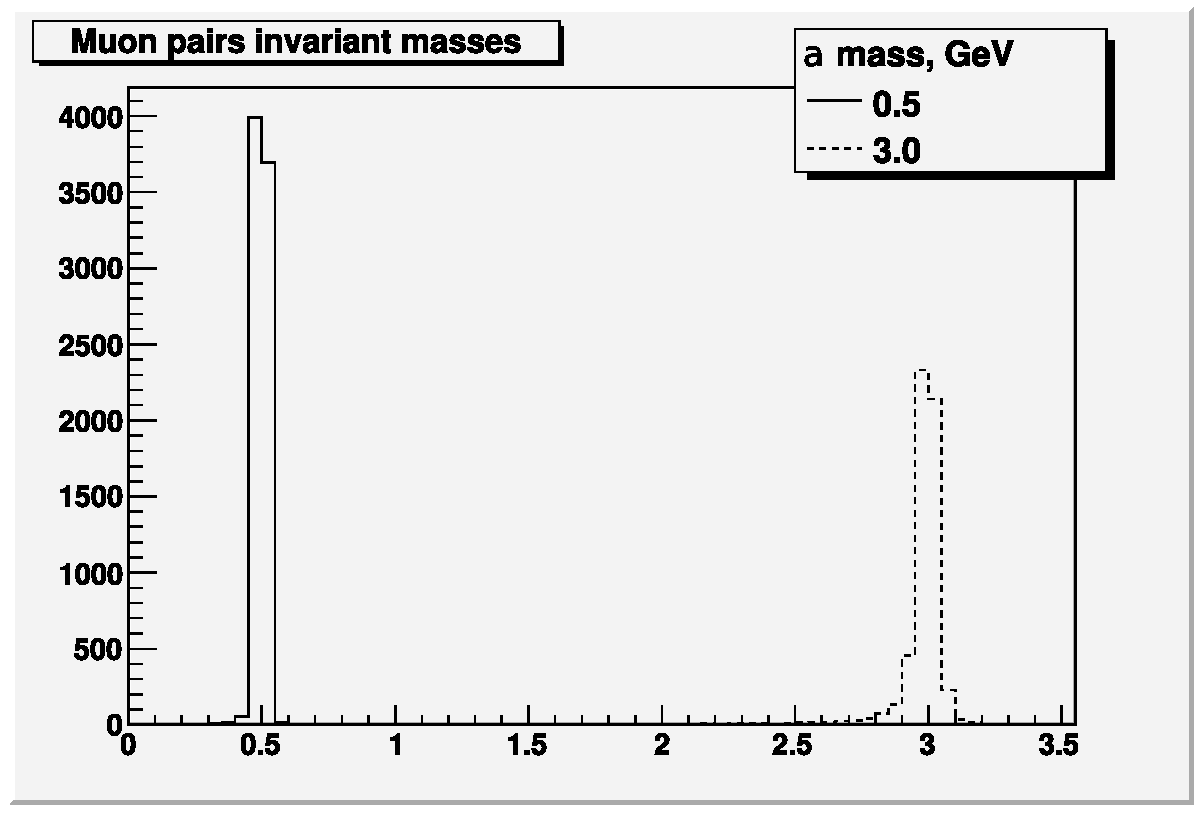
\includegraphics[width=0.5\linewidth]{muon_pairs_masses.pdf}
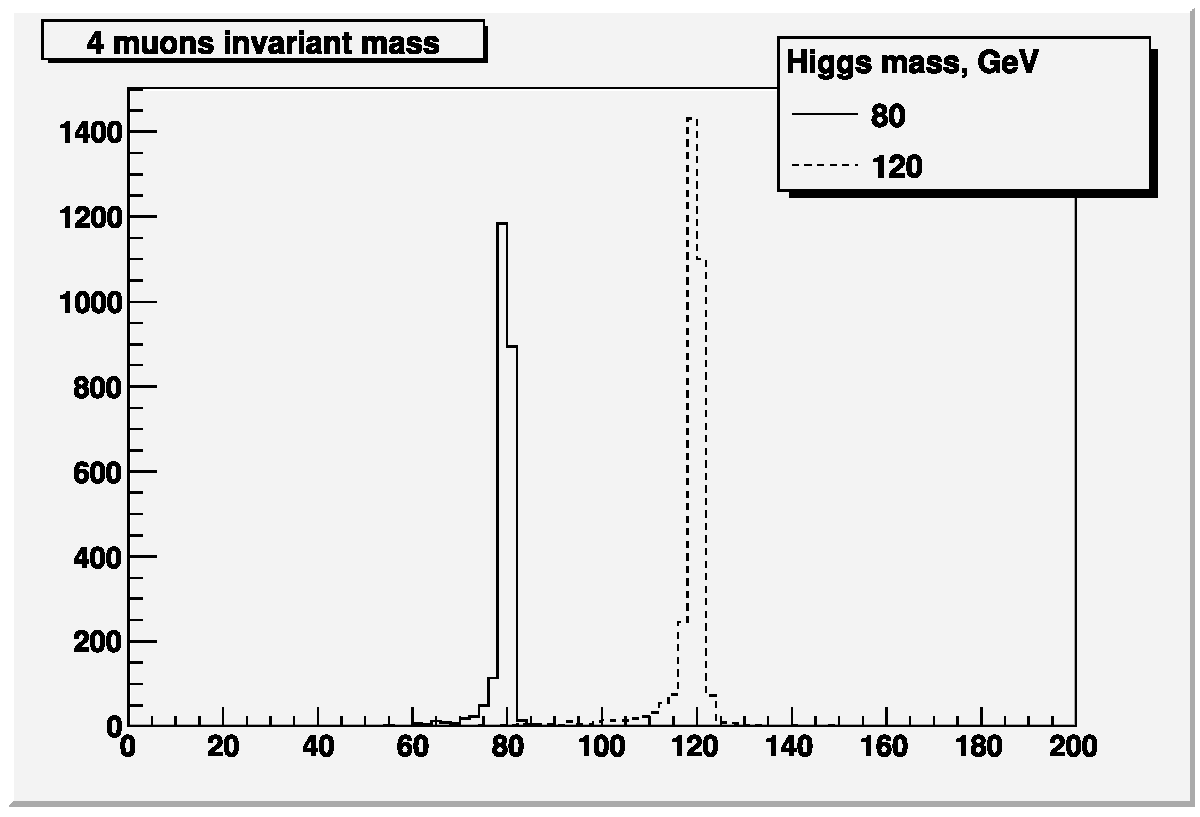
\includegraphics[width=0.5\linewidth]{invariant_mass.pdf}
\end{frame}

\begin{frame}
\frametitle{Acceptance}

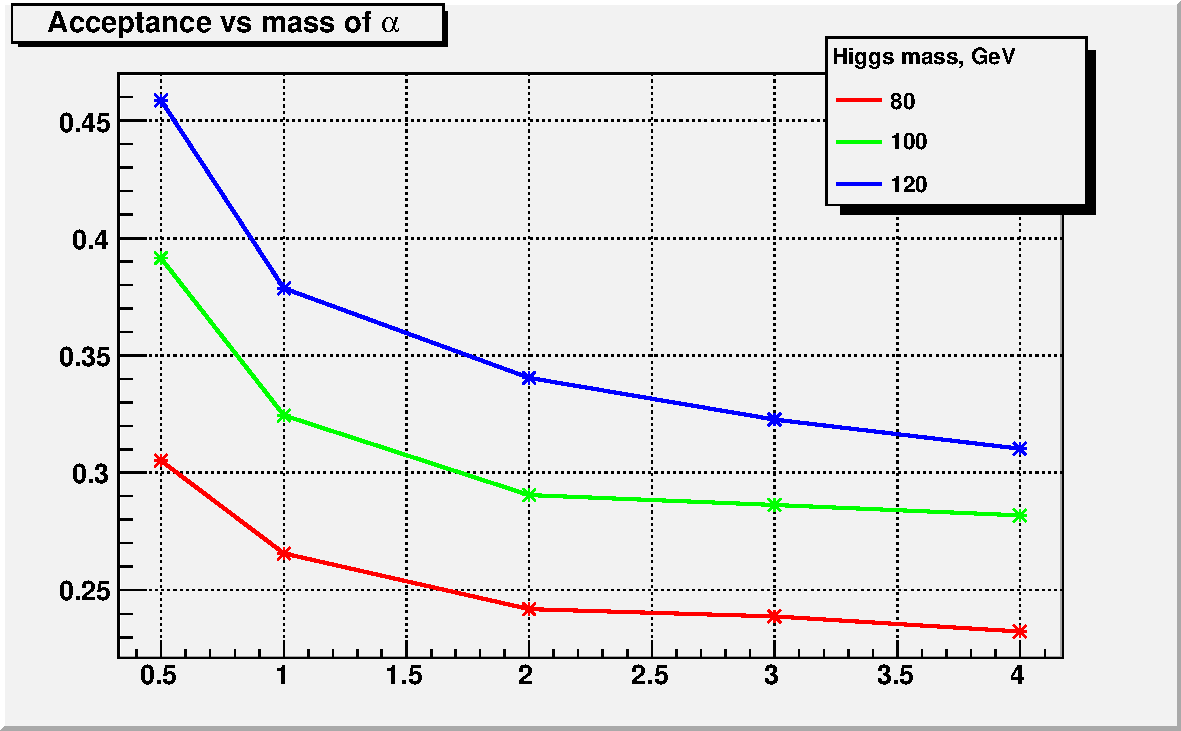
\includegraphics[width=0.5\linewidth]{acceptance_a.pdf}
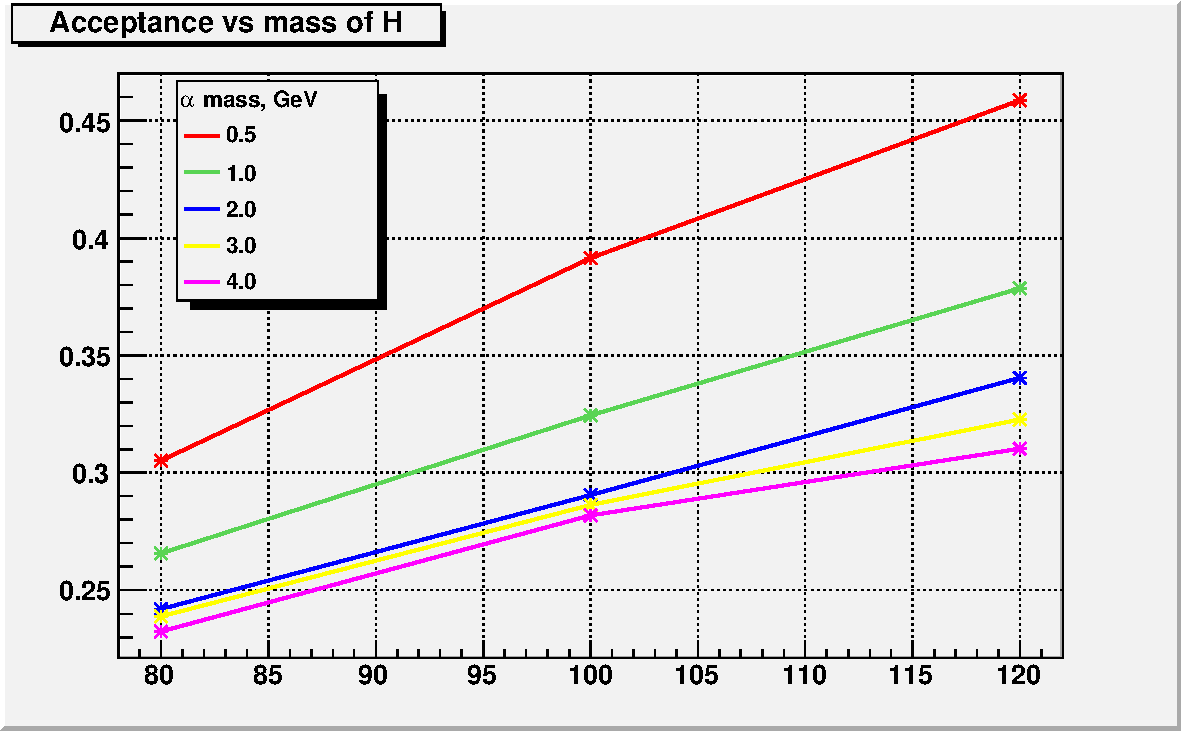
\includegraphics[width=0.5\linewidth]{acceptance_H.pdf}

\vspace{0.5 cm}
\hspace{-0.83 cm} \textcolor{darkblue}{\Large Backgrounds}

\vspace{-0.25 cm}
\renewcommand{\arraystretch}{1.5}
\begin{tabular}{c c c c}
& Inclusive $\mu + X$ & \mbox{\hspace{0.25 cm}}diboson/DY\mbox{\hspace{0.25 cm}} & \mbox{\hspace{0.25 cm}}$J/\psi$\mbox{\hspace{0.25 cm}} \\\hline
before cuts (100~pb$^{-1}$) & 150,000 & 48 & 120 \\
kinematic cuts on $4\mu$ & 150 & 5.9 & $0^{+0.07}_{-0.00}$ \\
effective region of fit$^*$ & $0^{+2.0}_{-0.0}$ & $0^{+0.005}_{-0.000}$ & \\
\end{tabular}

\vfill
$^*$fit sensitive to $m_{12}\mbox{, }m_{34} < 4$~GeV, $m_{1234} > 60$~GeV, and

\vspace{0.1 cm}
\textcolor{white}{$^*$fit sensitive to} $|m_{12} - m_{34}| < 0.08\mbox{ GeV} + 0.005 \, (m_{12} + m_{34})$
\end{frame}

\begin{frame}
\frametitle{Upper limits at low luminosity}

\vspace{0.5 cm}
\begin{columns}
\column{0.5\linewidth}
\begin{itemize}
\item Example likelihood function with no signal
\end{itemize}

\column{0.5\linewidth}
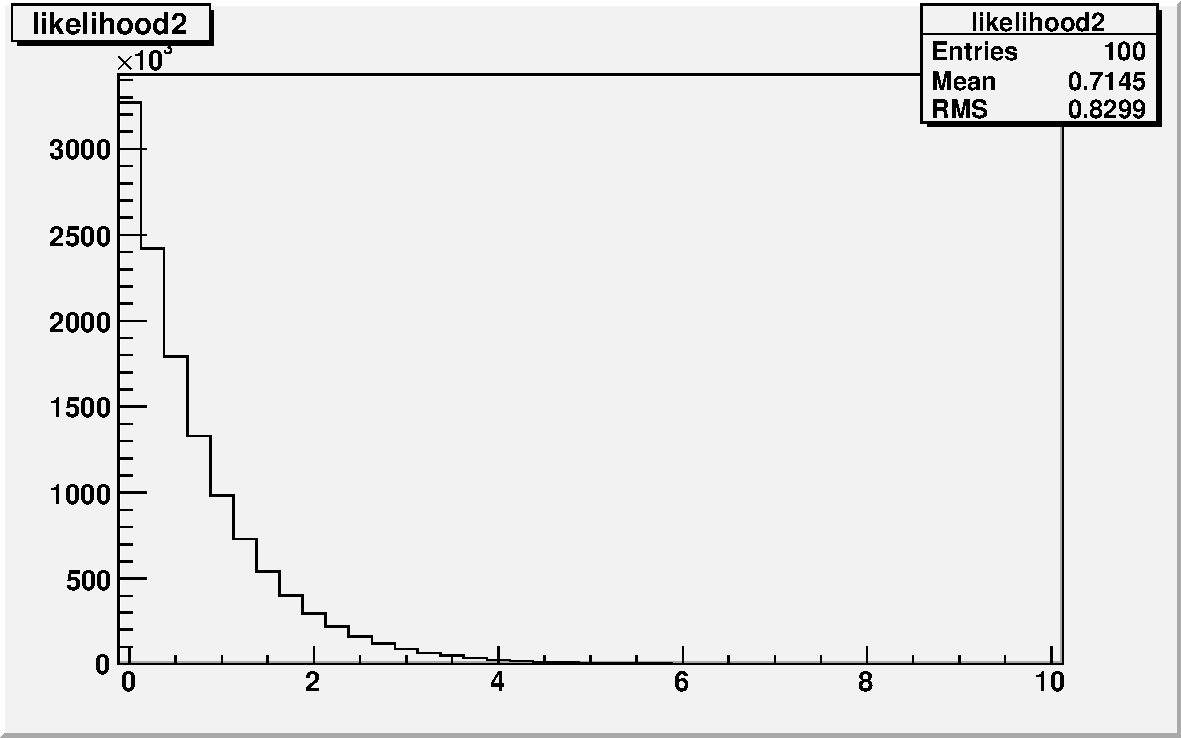
\includegraphics[width=\linewidth]{likelihood_NoSignal.pdf}
\end{columns}

\vspace{0.25 cm}
\begin{center}
95\% C.L.\ on $\sigma(pp \to h) \times \mathcal{B}(h \to aa)$ at $\mathcal{L} = 100$~pb$^{-1}$

\vspace{0.25 cm}
\renewcommand{\arraystretch}{1.5}
\begin{tabular}{c | c c c}
& $m_a = 1$~GeV & \mbox{\hspace{0.25 cm}}2~GeV\mbox{\hspace{0.25 cm}} & \mbox{\hspace{0.25 cm}}3~GeV\mbox{\hspace{0.25 cm}} \\\hline
$m_h = 80$~GeV & 10.9~pb & 4.1~pb & 4.6~pb \\
100~GeV & 8.9~pb & 3.4~pb & 3.8~pb \\
120~GeV & 7.7~pb & 2.9~pb & 3.4~pb \\
\end{tabular}
\end{center}
\end{frame}

%% \begin{frame}
%% \frametitle{Outline}
%% \begin{itemize}\setlength{\itemsep}{0.75 cm}
%% \item 
%% \end{itemize}
%% %% \hspace{-0.83 cm} \textcolor{darkblue}{\Large Outline2}
%% \end{frame}

%% \section*{First section}
%% \begin{frame}
%% \begin{center}
%% \Huge \textcolor{blue}{First section}
%% \end{center}
%% \end{frame}

\begin{frame}
\frametitle{Conclusions}

\begin{itemize}\setlength{\itemsep}{0.5 cm}
\item NMSSM solves naturalness problems in them MSSM, including tension from LEP Higgs limit
\item Introduces a rich Higgs sector with Higgs-to-Higgs decays
\item $h \to aa \to 4\mu$ is a sensitive discovery mode when $m_a < 2m_\tau$
\item D$\emptyset$ search doesn't rule out the $4\mu$ parameter space
\item CMS muon spectrometer allows for identification of all four muons
\end{itemize}

\label{numpages}
\end{frame}

\end{document}
